%%%%%%%%%%%%%%%%%%%%%%%%%%%%%%%%%%%%%%%%%
% Główny plik pracy
% Szablon pracy dyplomowej
% Wydział Informatyki 
% Zachodniopomorski Uniwersytet Technologiczny w Szczecinie
% autor Joanna Kołodziejczyk (jkolodziejczyk@zut.edu.pl)
% Bardzo wczesnym pierwowzorem szablonu był
% The Legrand Orange Book
% Version 2.1 (26/09/2018)
%
% Modifications to LOB assigned by %JK
%%%%%%%%%%%%%%%%%%%%%%%%%%%%%%%%%%%%%%%%%


%----------------------------------------------------------------------------------------
%	PAKIETY ORAZ PLIKI ZAWIERAJĄCE DEFINICJE STYLI I KONFIGURACJĘ OTOCZEŃ LATEX
%----------------------------------------------------------------------------------------

\documentclass[12pt,fleqn,twoside]{book} % JK Rozmiary czcionek są zgodne z wymaganiami uczelni 
% UWAGA! - wydruk jest dwustronny i jest to zabieg zamierzony

\usepackage{polski}
\usepackage[utf8]{inputenc}
\usepackage{graphicx}
\usepackage{multirow}
\usepackage{wrapfig}
\usepackage{pgfplots}
\graphicspath{ {images/} }

\usetikzlibrary{shadows}
\usetheme{Dresden}

 % JK - Plik zawierający podstawowe elementy konfigurujące układ dokumentu
% UWAGA! - raczej nie będzie potrzeby zmieniania jego struktury

%%%%%%%%%%%%%%%%%%%%%%%%%%%%%%%%%%%%%%%%%
% Plik z definicjami
% Szablon pracy dyplomowej
% Wydział Informatyki 
% Zachodniopomorski Uniwersytet Technologiczny w Szczecinie
% autor Joanna Kołodziejczyk (jkolodziejczyk@zut.edu.pl)
% Bardzo wczesnym pierwowzorem szablonu był
% The Legrand Orange Book
% Version 2.1 (26/09/2018)
%
% Modifications to LOB assigned by %JK
%%%%%%%%%%%%%%%%%%%%%%%%%%%%%%%%%%%%%%%%%



\def\HRule{\color{blueWI} \rule{\linewidth}{0.6pt}}

%----------------------------------------------------------------------------------------
% Typ pracy (wybrać właściwy)
%----------------------------------------------------------------------------------------
\def\degreename{praca dyplomowa magisterska} 
%\def\degreename{praca dyplomowa inżynierska}

%----------------------------------------------------------------------------------------
% Temat pracy
%----------------------------------------------------------------------------------------
%\def\ttitle{Szablon pracy dyplomowej inżynierskiej lub magisterskiej, do wykorzystania przez studentów Wydziału Informatyki Zachodniopomorskiego Uniwersytetu Technologicznego}
\def\ttitle{Projekt i implementacja kompilatora języka JavaScript na platformę .NET.}
\def\shorttitle{Projekt i implementacja kompilatora języka JavaScript na platformę .NET.} %Jeżeli tytuł pracy jest na tyle długi, że zajmuje 3 linijki to trzeba podać krótszy ekwiwalent do nagłówków stron parzystych
\def\ttitleEng{Design and implementation of the JavaScript compiler into the .NET platform.} %temat pracy w j. angielskim


%----------------------------------------------------------------------------------------
% Informacje o autorze
%----------------------------------------------------------------------------------------
\def\authornames{Przemysław Gawlas} %imię i nazwisko autora
\def\albumno{gp36035} %numer albumu
\def\speciality{Inżynieria oprogramowania} %nazwa specjalności
\def\field{Informatyka} %dziedzina nauki
\def\studyform{studia niestacjonarne} %forma studiów

%----------------------------------------------------------------------------------------
% Informacje o promotorze
%----------------------------------------------------------------------------------------
\def\supname{dr~inż.~Piotr~Błaszyński} %imię i nazwisko promotora
\def\departmentname{Katedra Inżynierii Oprogramowania i Cyberbezpieczeństwa} %nazwa katedry promotora

%----------------------------------------------------------------------------------------
% Data wydania tematu pracy
%----------------------------------------------------------------------------------------
\def\datetitle{05.10.2020}

%----------------------------------------------------------------------------------------
% Rok i miejsce złożenia pracy
%----------------------------------------------------------------------------------------
\def\placesubmit{Szczecin}
\def\yearsubmit{2021}
  % JK - dodatkowe definicje głównie treść strony tytułowej
% UWAGA! - konieczność edycji celem zmiany autora/tematu/dat itp., itd

%----------------------------------------------------------------------------------------
% OTWARCIE DOKUMENTU
%----------------------------------------------------------------------------------------
\begin{document}

%----------------------------------------------------------------------------------------
% STRONA TYTUŁOWA 
%----------------------------------------------------------------------------------------
\title
 {Projekt i implementacja kompilatora języka JavaScript na platformę .NET.}
\author[Przemysław Gawlas]
	{Przemysław Gawlas\\[3mm]Opiekun pracy: dr inż. Piotr Błaszyński}

\addtobeamertemplate{navigation symbols}{}{
    \usebeamerfont{footline}
    \usebeamercolor[fg]{footline}
    \hspace{1em}
    \insertframenumber/\inserttotalframenumber
}

\date{}

\begin{frame}
	\titlepage
\end{frame}


%----------------------------------------------------------------------------------------
% PUSTA STRONA PO STRONIE TYUŁOWEJ (JK - design and implementation)
%----------------------------------------------------------------------------------------
\newpage
\thispagestyle{empty}
~\vfill

%----------------------------------------------------------------------------------------
% STRONA Z OŚWIADCZENIEM AUTORA (JK - design and implementation)
%----------------------------------------------------------------------------------------
\newpage
\thispagestyle{empty}
%%%%%%%%%%%%%%%%%%%%%%%%%%%%%%%%%%%%%%%%%
% Strona z oświadczeniem wymaganym przez ZUT
% Szablon pracy dyplomowej
% Wydział Informatyki 
% Zachodniopomorski Uniwersytet Technologiczny w Szczecinie
% autor Joanna Kołodziejczyk (jkolodziejczyk@zut.edu.pl)
% Bardzo wczesnym pierwowzorem szablonu był
% The Legrand Orange Book
% Version 2.1 (26/09/2018)
%
% Modifications to LOB assigned by %JK
%%%%%%%%%%%%%%%%%%%%%%%%%%%%%%%%%%%%%%%%%


\begin{center}
\noindent 
{{\color{blueZUT}\Large\sffamily {Oświadczenie\\[.2cm]
autora pracy dyplomowej}}}\\[1cm] 
\end{center}

\noindent Oświadczam, że \degreename {\ }pn.{\ }{\emph \ttitle}{\ }
napisana pod kierunkiem \supname  {\ }
jest w całości moim samodzielnym autorskim opracowaniem sporządzonym przy wykorzystaniu wykazanej w pracy literatury przedmiotu i materiałów źródłowych. 
Złożona w dziekanacie Wydziału Informatyki
treść  mojej pracy dyplomowej w formie elektronicznej jest zgodna z treścią w formie pisemnej.

\vspace{0.2cm}

\noindent Oświadczam ponadto, że złożona w dziekanacie praca dyplomowa ani jej fragmenty nie były wcześniej przedmiotem procedur procesu dyplomowania związanych z uzyskaniem tytułu zawodowego w uczelniach wyższych.

\vspace{3.5cm}

\noindent {Podpis autora:}\dotfill % Printing/edition date

\vspace{1.5cm}

\noindent {Szczecin, dnia:\dotfill} % Printing/edition date

%----------------------------------------------------------------------------------------
%	STRESZCZENIE I SŁOWA KLUCZOWE (1 STRONA) (JK - design and implementation)
%----------------------------------------------------------------------------------------
\newpage
\thispagestyle{empty}
%%%%%%%%%%%%%%%%%%%%%%%%%%%%%%%%%%%%%%%%%
% Specjalna strona pracy ze streszczeniem i abstractem w j. angielskim
% Szablon pracy dyplomowej
% Wydział Informatyki 
% Zachodniopomorski Uniwersytet Technologiczny w Szczecinie
% autor Joanna Kołodziejczyk (jkolodziejczyk@zut.edu.pl)
% Bardzo wczesnym pierwowzorem szablonu był
% The Legrand Orange Book
% Version 2.1 (26/09/2018)
%
% Modifications to LOB assigned by %JK
%%%%%%%%%%%%%%%%%%%%%%%%%%%%%%%%%%%%%%%%%


\begin{center}
\noindent {{\color{blueZUT}\Large\sffamily  {Streszczenie}}}\\[1cm] 
\end{center}
Celem niniejszej pracy było zaprojektowanie oraz implementacja kompilatora języka JavaScript platformę .NET. Praca przedstawia dostępne narzędzia, technologie oraz języki programowania wykorzystane w projekcie oraz technologie pokrewne które mogły by być wykorzystane. Przedstawia częściową analizę języka JavaScript na podstawie której wyznaczany jest zakres implementacji kompilatora. Praca przedstawia projekt oraz wyjaśnia implementację kompilatora. W celu weryfikacji poprawności działania, zostały przygotowane programy testujące.

\vspace{10pt}
\noindent{\bf słowa kluczowe:} kompilator, JavaScript, .NET

\vfill

\begin{center}
\noindent {{\color{blueZUT}\Large\sffamily {Abstract}}}\\[1cm] 
\end{center}
The aim of this diploma thesis was to design and implement a JavaScript language compiler for .NET platform. The work presents the available tools, technologies and programming languages used in the project and related technologies that could be used. It presents a partial analysis of the JavaScript language on the basis of which the scope of the compiler implementation is determined. The work presents the project and explains the implementation of the compiler. In order to verify the correctness of operation, testing programs have been prepared. 

\vspace{10pt}
\noindent{\bf keywords:} compiler, JavaScript, .NET
 %abstract.tex 
 
%----------------------------------------------------------------------------------------
%	SPIS TREŚCI (JK - design and implementation)
%----------------------------------------------------------------------------------------
\pagestyle{empty}  % Wyłącz stopkę i nagłówek w TOC
\tableofcontents % wyświetl spis
\addtocontents{toc}{\protect\thispagestyle{empty}} % Zachowaj pusty nagłówek i stopkę w TOC
% Wymuszenie rozpoczęcie pierwszego rozdziału na nieparzystej stronie, aby znajdował się po prawej stronie 
\cleardoublepage 
% Ponownie włącz nagłówki i stopki
\pagestyle{fancy} 

%----------------------------------------------------------------------------------------
%	WSTĘP W PRACY DYPLOMOWEJ (JK - design and implementation)
%----------------------------------------------------------------------------------------
\addcontentsline{toc}{chapter}{Wstęp}
%%%%%%%%%%%%%%%%%%%%%%%%%%%%%%%%%%%%%%%%%
% Plik z wstępem do pracy
% Szablon pracy dyplomowej
% Wydział Informatyki 
% Zachodniopomorski Uniwersytet Technologiczny w Szczecinie
% autor Joanna Kołodziejczyk (jkolodziejczyk@zut.edu.pl)
% Bardzo wczesnym pierwowzorem szablonu był
% The Legrand Orange Book
% Version 2.1 (26/09/2018)
%
% Modifications to LOB assigned by %JK
%%%%%%%%%%%%%%%%%%%%%%%%%%%%%%%%%%%%%%%%%


\chapter*{Wstęp}

\par W branży programistycznej istnieje bardzo dużo języków programowania oraz różnych środowisk uruchomieniowych dla nich przeznaczonych. Podczas tworzenia oprogramowania niezbędny jest dla programisty kompilator. Zamienia on kod programu napisanego w konkretnym języku programowania, na zrozumiały dla środowiska uruchomieniowego ciąg instrukcji. Warto podkreślić, że języki programowania, które są proste do zrozumienia i opanowania dla programistów oraz pozwalają na pisanie programów, które można uruchomić na różnych urządzeniach i umożliwiają tworzenie bardzo zróżnicowanych rodzajów oprogramowania, są o wiele częściej używane niż inne. Powoduje to, że powstaje dużo różnych bibliotek i frameworków ułatwiających i automatyzujących tworzenie oprogramowania.

\par Jednym z popularnych języków wśród programistów jest język JavaScript, który może być uruchomiany w przeglądarkach internetowych lub w maszynie wirtualnej takiej jak Node.js. Innym z popularnych środowisk uruchomieniowych jest platforma .NET, dla której istnieje wiele kompilatorów różnych języków. Wykorzystanie istniejących bibliotek, frameworków czy modułów napisanych w języku JavaScript w niezmienionej formie na platformie .NET, umożliwi programistom na tworzenie bardziej uniwersalnego kodu.

\par \textbf{Celem} niniejszej pracy jest \textbf{zaprojektowanie} oraz \textbf{implementacja kompilatora} języka \textbf{JavaScript} na kod \textbf{IL Assembler} uruchamiany na \textbf{platformie .NET}. Następnie w celu sprawdzenia poprawności działania kompilatora, zostaną przeprowadzone testy przy pomocy prostych implementacji kodu JavaScript. Zostaną również zaprojektowane oraz zaimplementowane dwa bardziej skomplikowane testy, do \textbf{porównania maszyn wirtualnych Node.js oraz .NET}. Zostanie także porównany kod assemblera generowanego przez kompilator .Net Core języka C\# z kodem generowanym przez implementowany kompilator.

\par Praca podzielona jest na cztery części. Pierwsza część opisuje pojęcia i technologie wykorzystywane do realizacji tego projektu oraz technologie pokrewne, które w pewnym stopniu realizują cel pracy lub realizują podobne założenia. Druga część poświęcona jest zaprojektowaniu tworzonego kompilatora. Kolejna część opisuje sposób implementacji tego kompilatora na podstawie zdefiniowanych założeń. Ostatnia część opisuje przeprowadzone testy realizowane w ramach pracy oraz przedstawia wyniki ich działania.
 % introduction.tex zawiera treść wstępu

%----------------------------------------------------------------------------------------
%	ROZDZIAŁ 1
%----------------------------------------------------------------------------------------
\chapter{Pojęcia i technologie}
\label{rozdzial1}

\section{Zakres projektu}
\index{Zakres projektu}

Projekt będzie realizował zaprojektowanie i implementację kompilatora języka JavaScript na platformę uruchomieniową .NET core. W tym rozdziale zostaną opisane pojęcia oraz technologie, które będą wykorzystywane w realizacji tego projektu. Na początku opisane będą takie pojęcia jak \textit{kompilator} oraz \textit{maszyna wirtualna}. Następie zostaną omówione technologie wiodące w projekcie takie jak \textit{JavaScript}, \textit{Node.js}, \textit{.NET Core} oraz \textit{IL Assembler}.

\subsection{Kompilator}
\index{Kompilator}
W dzisiejszych czasach niezbędnym narzędziem programisty jest kompilator. Jest to narzędzie, którego zadaniem jest tłumaczenie programu napisanego przez programistę, na program który będzie można uruchomić na konkretnym środowisku uruchomieniowym.
\par Mówiąc ściślej kompilator to program napisany w języku implementacyjnym, który odczytuje język źródłowy i tłumaczy go na język wynikowy. Proces zamiany kodu źródłowego na wynikowy nazywany jest \textbf{kompilacją}. Kodem wynikowym procesu kompilacji może być od razu kod maszynowy, który interpretowany jest bezpośrednio przez procesor lub maszynę wirtualną, albo do kodu pośredniego, który też może zostać skompilowany przez inny kompilator.
\par Kompilatory mogą być napisane w dowolnym języku programowania. Istnieje kilka specjalnie zaprojektowanych do tego zadania języków, takie jak \textit{Pascal} czy \textit{Algol 68}. Nie mniej jednak, wybór języka do implementacji kompilatora przez twórcę, powinien się opierać na założeniu, że powinien on zminimalizować wysiłek implementacyjny i zmaksymalizować jakość kompilatora.
\par Język źródłowy który przetwarzany jest przez kompilator prawie zawsze jest oparty na wcześniej zdefiniowanej gramatyce. Dzięki temu program kompilatora potrafi odróżnić od siebie kolejne instrukcje i zamienić je na równoważne ciągi instrukcji w języku docelowym.
\footcite[1-4]{Mckeeman1974}
\par Podobnym w działaniu jest \textbf{interpreter}, który tak jak kompilator, jest pisany w jednym implementacyjnym oraz odczytuje język kodu źródłowego, ale nie produkuje kodu wynikowego, tylko odczytany kod jest od razu wykonywany. Niektóre języki przyjmują schematy zawierające wykorzystanie kompilatora oraz interpretera w procesie wytwarzania oprogramowania. Jednym z przykładów jest język \textbf{Java}, który kompilowany jest do postaci nazywanej \textit{bytecode}, a następnie interpretowany jest przez maszynę wirtualną Java (Java Virtual Machine, JVM).\footcite[3,4]{EngineeringCompiler}

\subsection{Maszyna wirtualna}
% https://ieeexplore.ieee.org/stamp/stamp.jsp?tp=&arnumber=1430629

\par Wirtualizacja stała się ważnym narzędziem w projektowaniu systemów komputerowych, a maszyny wirtualne używane są w wielu obszarach informatycznych, od systemów operacyjnych po architektury procesorów języków programowania.
\par Dla programistów oraz użytkowników wirtualizacja likwiduje tradycyjne interfejsy oraz ograniczenia zasobów związanych z różnymi urządzeniami. Maszyny wirtualne zwiększają interoperacyjność oprogramowania oraz wszechstronność platformy, dlatego też często się je wykorzystuje.
\par Maszyna wirtualna to nic innego jak program uruchamiany na prawdziwej maszynie, który potrafi obsługiwać pożądaną architekturę. W ten sposób można obejść rzeczywistą kompatybilność maszyny i ograniczenia zasobów sprzętowych. Pozwala to, między innymi na równoczesne tworzenie oprogramowania dla wielu platform, bez konieczności stosowania bezpośrednio interfejsów rzeczywistej maszyny, a jedynie wykorzystanie tych udostępnianych przez maszynę wirtualną. \footcite{Smith2005}

\subsection{JavaScript}
Jest to skryptowy język programowania, dzięki którego można realizować aplikacje w paradygmacie imperatywnym, obiektowym oraz funkcyjnym. Najczęściej jest wykorzystywany w stronach internetowych, gdzie kolejne instrukcje wykonywane są przez przeglądarkę sieci Web, ale również zyskuje popularność w innych środowiskach. \footcite{aboutJS}
\par JavaScript został wdrożony w roku 1995 roku, jako sposób dodawania programów do stron internetowych. Jako pierwszą przeglądarką obsługującą JavaScript to Netscape Navigator. Następnie inne, głównie graficzne przeglądarki wprowadzały możliwość uruchamiania kodu napisanego w JavaScript. Umożliwiło to tworzenie nowoczesnych stron internetowych z którymi można było bezpośrednio współpracować, bez konieczności ponownego pobierania strony po każdej wykonanej akcji.
\par W momencie kiedy zaczęto używać JavaScript poza Netscape, został stworzony dokument standaryzujący, który opisuje sposób działania języka. Utworzono go, aby wszystkie nowo tworzone oprogramowanie mające wykorzystywać JavaScript, faktycznie używały tego samego języka. Dokument ten nazywany jest standardem \textbf{ECMAScript}, który został nazwany po organizacji Ecma International, twórców tego dokumentu.
\par JavaScript jest językiem bardzo elastycznym, przez co ma też swoje wady i zalety. Przez swoją elastyczność pozwala na wykorzystywanie wielu technik i praktyk programistycznych które mogą być niemożliwe w innych językach.
\par Jako, że jest to język skryptowy, to tak jak podobne tego typu języki posiada dynamiczne typowanie zmiennych. Oznacza to, że każda ze zmiennej jest definiowana poprzez słowo kluczowe \texttt{var}, a w nowszej wersji można to zrobić już przy pomocy dwóch różnych słów \texttt{const} oraz \texttt{let}. Kolejną z podstawowych rzeczy w JavaScript są funkcje. Dzięki nim można pisać programy we wspomnianych wcześniej paradygmatach. Pozwalają one nie tylko na wydzielenie kodu na mniejsze części ale również na definiowanie bardziej złożonych struktur czy klas.\footcite{EloquentJavaScript}
% https://eloquentjavascript.net/Eloquent_JavaScript.pdf

\subsection{Node.js}
Jest to asynchroniczne środowisko uruchomieniowe dla języka JavaScript. Node.js został zaprojektowany do tworzenia skalowalnych aplikacji sieciowych. Pozwala na jednoczesne przetwarzanie wielu połączeń. Przy każdym połączeniu następuje wywołanie zwrotne, a w przypadku jeśli nie będzie żadnej pracy do wykonania, Node.js przejdzie w tryb uśpienia.
\footcite{Node.js2017}

\par Środowisko Node.js oparte jest na implementacji silnika ``V8'' stworzonego przez Google. Zaimplementowany głownie jest w języku C i C++, koncentrując się na wydajności i niskim zużyciu pamięci. Różnica polega na tym, że silnik ``V8'' obsługuje głównie JavaScript w przeglądarkach internetowych, a Node.js został stworzony z myślą o obsłudze długotrwałych procesów serwerowych.
\par W celu obsługi jednoczesnego wykonywania logiki biznesowej, Node.js opiera się na asynchronicznym modelu zdarzeń wejścia i wyjścia, w przeciwieństwie do większości innych współczesnych środowisk, które oparte są na wielowątkowości. Model zdarzeń jest obsługiwany na poziomie języka, a jest to możliwe ponieważ JavaScript obsługuje wywołania zwrotne zdarzeń oraz funkcjonalny charakter JavaScript sprawia, że niezwykle łatwo jest tworzyć anonimowe obiekty funkcji, które można zarejestrować jako programy obsługi zdarzeń. \footcite{Tilkov2010}

\subsection{.NET Core}

\par Jest to platforma programistyczna ogólnego zastosowania z otwartymi kodami źródłowymi. Pozwala na tworzenie aplikacji dla systemów Windows, macOS oraz Linux przy wykorzystaniu różnych języków programowania.\footcite{dotNetvsFramework}
\par Architektura środowiska .NET składa się z takich komponentów jak:
\begin{itemize}
  \item CTS (Common Type System) - opisuje wszystkie wspierane przez platformę typy. Definiuje zasady korzystania z danych typów, dostarcza zorientowany obiektowo model dla różnych języków implementowanych w .NET oraz zapewnia bibliotekę zawierającą prymitywne typy danych (takich jak \texttt{Boolean}, \texttt{char} itp.).
  \item CLS (Common Language Specyfication) - definiuje w jaki sposób mają być definiowane obiekty i funkcje, w języku przeznaczonym na platformę .NET. CLS jest podzbiorem CTS, co oznacza, że wszystkie opisane zasady CTS dotyczą również CLS.\footcite{dotNetCLS}
  \item FCL (Framework Class Library) - jest to standardowa biblioteka zawierająca podstawę implementacji klas, interfejsów, typów wartości czy usług, które wykorzystywane są do tworzenia aplikacji.\footcite{dotNetFCL}
  \item CLR (Common Language Runtime) - jest to środowisko uruchomieniowe, które uruchamia kod i zapewnia usługi ułatwiające proces programowania. Środowisko wykonawcze automatycznie obsługuje układ obiektów i zarządza referencjami no nich, zwalniając je w przypadku kiedy już nie są używane.\footcite{dotNetCLR}
  
\end{itemize}

\subsection{IL Assembler}
\par Każdy z kompilatorów przeznaczonych na platformę .NET, bez względu na wybrany język, kompiluje kod do postaci pośredniej, jakim jest kod IL.
\par Wykonywalny kod IL jest w formacie binarnym i nie jest czytelny dla człowieka. Oczywiście jak inne wykonywalne kody binarne, mogą zostać przedstawione w postaci assemblera, tak i kod IL może zostać zaprezentowany w postaci IL Assemblera. Zestaw instrukcji jest taki jak w przypadku tradycyjnego assemblera. Przykładowo, aby dodać dwie liczby należy użyć instrukcji \texttt{add}, a w przypadku odejmowania, należy użyć instrukcji \texttt{sub}.
\par Środowisko uruchomieniowe .NET nie potrafi jednak odczytywać bezpośrednio IL Assemblera. Aby kod napisany w IL Assemblerze można było uruchomić, trzeba skompilować go do postaci binarnej IL. \footcite{ILAsm1}

\section{Technologie pokrewne}
Aktualnie istnieje wiele rozwiązań przetwarzających język JavaScript jak i narzędzi, dzięki którymi można budować, jak i uruchamiać aplikacje dedykowane na platformę .NET. W tym rozdziale zostaną opisane niektóre z tych technologii.

\subsection{JScript}
\par Jest to język programowania opracowany przez firmę \textbf{Microsoft} w oparciu o wczesne standardy języka JavaScript. Podstawową i największą różnicą, która wyróżnia język JScript jest to, że nie jest to prosty język skryptowy. Pozwala on na tworzenie w pełni funkcjonalnych aplikacji jako pliki wykonywalne, które można bezpośrednio uruchamiać na komputerach klienckich. \footcite{jscript}

% \subsection{ActionScript}
% Obiektowy język oparty na ECMAScript używany w Adobe Flash/

\subsection{TypeScript}
\par Jest to język programowania o otwartym kodzie, który opiera się na JavaScript. Wzbogaca składnię JavaScript o statyczne definicje typów. Definiowane typy umożliwiają opisanie kształtu obiektów, tworzenie lepszej dokumentacji kodu oraz sprawdzanie poprawności kodu jeszcze przed jego uruchomieniem. 
\par Kod TypeScript jest przekształcany na kod JavaScript przy pomocy kompilatora \textit{TypeScript} lub \textit{Babel}. Przekształcony kod może być uruchamiany jako zwykły JavaScript na przeglądarkach czy też na maszynie wirtualnej Node.js. \footcite{typescript}

% \subsection{?CoffeeScript}
% Język programowania kompilowany do JavaScript.
% Nie wiem czy warto wspominać.

% Inne języki kompilowane do JavaScript: Roy, Kaffeine, Clojure, Opal

\subsection{Babel}
\par Jest to transkompilator języka JavaScript pozwalający na transpilacje nowych funkcjonalności do starego standardu. Dzięki temu narzędziu można między innymi na uruchomienie kodu zarówno w nowych, jak i starych przeglądarkach. Zawiera wiele opcji konfiguracji, które poza zmianą samych funkcjonalności \textit{JavaScript}, pozwala również zamienić kod \textit{TypeScript} czy kod \textit{React} do kodu \textit{JavaScript}. \footcite{babel}

\subsection{Deno}
\par Jest to środowisko uruchomieniowe pozwalające uruchamiać kod dla JavaScript oraz TypeScript. Stworzone zostało w oparciu o silnik \textit{JavaScript V8} oraz języku programowania \textit{Rust}. Deno jest oprogramowaniem o otwartym kodzie, które ma być wydajnym i bezpiecznym środowiskiem skryptowym. \footcite{deno}

% \subsection{asm.js}
% Jeśli dobrze zrozumiałem jest to okrojony JavaScript który tak samo może być uruchamiany w przeglądarkach czy Node.js/Deno.
% Wykorzystywany przy kompilacji kodu c++ do uruchamiania na tych maszynach.

\subsection{Emscripten}
Jest to kompilator o otwartych źródłach, pozwalający kompilować kod w języku \textit{C\\C++} do \textit{WebAssembly} oraz uruchamiać go w przeglądarkach internetowych, \textit{Node.js} lub innych środowiskach uruchomieniowych \textit{WebAssembly}. 
\par Praktycznie każda przenośna baza kodu \textit{C} lub \textit{C++} może zostać skompilowana do WebAssembly przy użyciu \textit{Emscripten}, począwszy od gier o wysokiej wydajności, które muszą renderować grafikę, odtwarzać dźwięki oraz ładować i przetwarzać pliki, aż po frameworki aplikacji, takie jak \textit{Qt}. \footcite{emscripten}


% \subsection{WebAssembly}
% % https://devenv.pl/webassembly-nadciaga-rewolucja/
% Język niskopoziomowy, który działa z szybkością zbliżoną do rozwiązań natywnych i pozwala na kompilację kodu napisanego w C/C++ do kodu binarnego działającego w przeglądarce internetowej.
% (Pomija JavaScript).

\subsection{C\#}
Czy opisywać rodzinę .NET?

Na maszynę .NET istnieją implementacje języków takich jak Python, Java, C++ i inne.

\subsection{.NET Framework}
Platforma programistyczna.

\subsection{Mono}
Implementacja open source platformy .NET Framework.

\subsection{DotGNU}
Alternatywa dla Mono.

\subsection{?Roslyn}
.NET Compiler Platform


 % chapter1.tex zawiera treść rozdziału 1

%----------------------------------------------------------------------------------------
%	ROZDZIAŁ 2
%----------------------------------------------------------------------------------------
\chapter{Projekt kompilatora}
\label{rozdzial2}
\section{Środowisko i narzędzia}
\par Kod kompilatora zostanie zrealizowany w języku \textit{C\#} na platformie \textit{.NET Core 3.1}. W projekcie zostanie również wykorzystana platforma \textit{.NET Framework} w celu dekompilacji skompilowanego kodu testów, ich kompilacji z kodu \textit{IL Assembler} oraz kompilacji kodu \textit{JScript}. W celu weryfikacji poprawności kodu \textit{JavaScript} zostanie wykorzystana platforma \textit{Node.js} w wersji 10.15. Zostanie również wykorzystany skrypt pomocniczy w \textit{PowerShell} służący do łatwego przeprowadzenia testów oraz do zebrania informacji o wielkości plików wykonywalnych i pomiaru czasu wykonania programów testowych. Drugim z dekompilatorów jaki zostanie wykorzystany w projekcie jest program \textit{JetBrains dotPeek 2020.2.1}. Ostatnim z programów, służący do pomiarów zużycia pamięci, jest \textit{JetBrains dotMemory 2020.2.1}.
\par Wszystkie testy oraz pomiary zostaną przeprowadzone na komputerze o następujących parametrach:
\begin{itemize}
  \item System operacyjny: Windows 10 Home
  \item Typ systemu: 64-bitowy
  \item Procesor: Intel(R) Core(TM) i7-4700MQ CPU @ 2.40Hz
  \item Pamięć RAM: 16 GB
\end{itemize}

\section{Analiza języka JavaScript i określenie zakresu implementacji}
% Opis składni JavaScript.
% Implementacja JavaScript w standardzie ES5.
% Musi być Turing-complete. Dodatkowo implementacja funkcji.

\par W tym rozdziale zawarty zostanie zakres implementacji oraz opis poszczególnych elementów języka JavaScript. W projekcie zostanie zaimplementowana jedynie część standardu ECMAScript, a niektóre mechanizmy zostaną uproszczone.

% #PYTANIE Czy warto opisać rzeczy które nie będą implementowane?

\subsection{Wyrażenia}

\par Składnia języka JavaScript zapożycza wiele rozwiązań użytych w Javie, jednak na konstrukcję miały też wpływ takie języki jak: Awk, Perl i Python. W języku JavaScript instrukcję nazywane są wyrażeniami, które rozdzielane są znakiem średniaka. Znaki białe takie jak spacja, tabulator czy znak końca linii nie mają wpływu na sposób działania kolejnych elementów wyrażeń, stanowią jedynie sposób ich oddzielenia. W kodzie źródłowym JavaScript rozróżnialna jest wielkość liter oraz wspierany jest standard znaków Unicode. ECMAScript definiuje również zestaw słów kluczowych i literałów oraz zasady automatycznego umieszczania średników ASI (Automatic semicolon insertion).

\subsection{Komentarze}

\par Rozróżniane są dwa typy komentarzy:
\begin{enumerate}
  \item Jednoliniowy - definiowany jest przy pomocy znaku ``$//$'' oraz umieszczany jest na końcu linii.
  \begin{lstlisting}[language=JavaScript, caption=Przykład komentarza jednoliniowego, label=alg:komentarze1]
    console.log(); // komentarz
  \end{lstlisting}
  \item Wieloliniowy - zawarty jest pomiędzy dwoma elementami ``/*'' oraz ``*/''
  \begin{lstlisting}[language=JavaScript, caption=Przykład komentarza wieloliniowego, label=alg:komentarze2]
    console.log();
    /*
      komentarz na
      wiele linii
    */
  \end{lstlisting}
\end{enumerate}

\subsection{Deklaracje zmiennych i stałych}
\par Zmienne deklaruje się przy pomocy słów kluczowych \texttt{var}, \texttt{let} oraz \texttt{const}. Deklaracja przy pomocy \texttt{var} jest podstawowym sposobem tworzenia zmiennych w JavaScript. Zasięg takiej zmiennej nie może być ograniczony przez blok w którym jest zawarta, przez co może powodować błędy przy pisaniu kodu. W celu uściślenia zasięgu i przeznaczenia zmiennych powstały dwa inne sposoby deklaracji \texttt{let} oraz \texttt{const}. Oba te rodzaje deklaracji powodują, że zakres dostępności zmiennej jest ograniczony do bloku w którym została zadeklarowana. Różnicą między tymi dwoma deklaracjami jest taka, że przy pomocy \texttt{const} definiujemy stałą która musi być od razu zadeklarowana, a \texttt{let} działa podobnie jak \texttt{var}.
\begin{lstlisting}[language=JavaScript, caption=Przykład deklaracji zmiennych, label=alg:deklaracjaZmiennej1]
  var zmienna1;
  let zmienna2;
  const stala = true;
\end{lstlisting}
\par Przy deklaracji zmiennych przy użyciu \texttt{var} lub \texttt{let}, dla których nie przypiszemy żadnej wartości, przyjmują one wartość \texttt{undefined}

\subsection{Typy danych}
% https://developer.mozilla.org/pl/docs/Web/JavaScript/Guide/Sk%C5%82adnia_i_typy
\par W najnowszym standardzie ECMAScript zdefiniowanych jest siedem typów danych:
\begin{enumerate}
  \item \texttt{Boolean} - może przybierać dwie wartości \texttt{true} lub \texttt{false}.
  \item \texttt{null} - słowo kluczowe oznaczające wartość zerową. 
  \item \texttt{undefined} - wartość nieokreślona.
  \item \texttt{Number} - tym przeznaczony dla literałów całkowitych jak i zmiennoprzecinkowych.
  \item \texttt{String} - typ przeznaczony dla literałów łańcuchowych reprezentujących zero lub więcej pojedynczych znaków ujętych w podwójny lub pojedynczy cudzysłów.
  \item \texttt{Symbol} - wprowadzony w ECMAScript 6 typ danych, który pozwala na tworzenie unikalnych i nie zmiennych wartości.
  \item \texttt{Object} - typ złożony do którego zaliczają się funkcje, tablice, słowniki oraz instancje klas.
\end{enumerate}

\subsection{Operacje arytmetyczne}
% https://developer.mozilla.org/en-US/docs/Web/JavaScript/Guide/Expressions_and_Operators
Operatory arytmetyczne przyjmują jako operandy wartości liczbowe w postaci literałów lub zmiennych i jako wynik zwracają pojedynczą wartość liczbową. Standardowe operatory arytmetyczne to:
\begin{itemize}
  \item dodawanie ``\texttt{+}''
  \item odejmowanie ``\texttt{-}''
  \item mnożenie ``\texttt{*}''
  \item dzielenie ``\texttt{/}''
\end{itemize}

\begin{lstlisting}[language=JavaScript, caption=Przykład użycia operatorów arytmetycznych, label=alg:operatoryArytmetyczne1]
  var v1 = 10 + 15
  var v2 = 100 + 100 / 2 * 3 + 10
  var v3 = 100.7 + 10.40 / 1.67 * 3.1 + 10.23
\end{lstlisting}


\subsection{Operacje porównania}
  \par Operatory porównania porównuje swoje operandy czego wynikiem jest wartość logiczna, określająca czy dane stwierdzenie jest prawdziwe. Operandy mogą być wartościami liczbowymi, łańcuchami znaków, logicznymi lub wartościami obiektu. W przypadku kiedy dwa operandy są różnego typu, JavaScript próbuje przekonwertować je na odpowiedni typ do porównania.
  \par Operatory porównania w języku JavaScript to:
  \begin{itemize}
    \item równość ``==''
    \item nierówność ``!=''
    \item ścisła równość ``===''
    \item ścisła nierówność ``!==''
    \item większy ``>''
    \item większy lub równy ``>=''
    \item mniejszy ``<''
    \item mniejszy lub równy ``<=''
  \end{itemize}
  Tutaj warto zauważyć, że JavaScript posiada dwa operatory równości i nierówności. Różnica pomiędzy ścisłym porównaniu a zwykłym polega na tym, że w przypadku kiedy operandy są różnego typu, to dla zwykłego porównywania, JavaScript próbuje przekonwertować wartości do jednego typu. Przy porównywaniu ścisłym nie zachodzi konwersja.

  \begin{lstlisting}[language=JavaScript, caption=Przykład użycia operatorów porównania, label=alg:operatoryPorownania1]
    var v1 = 2 == 2
    var v2 = 1 + 1 != 2
    var v3 = zmienna1 > zmienna2
  \end{lstlisting}

\subsection{Instrukcje warunkowe}
% https://developer.mozilla.org/pl/docs/Web/JavaScript/Guide/Control_flow_and_error_handling
Instrukcje warunkowe to zbiór instrukcji, których wykonanie jest zależne od zdefiniowanego warunku którego wynikiem jest wartość logiczna ``true'' lub ``false''. JavaScript wspiera dwa rodzaje instrukcji warunkowych:
\begin{itemize}
  \item \texttt{if .. else}
  \item \texttt{siwtch}
\end{itemize}
\par Instrukcja \texttt{if} wykonuje blok instrukcji w przypadku, kiedy podany warunek zwróci wartość ``true''. Jeśli trzeba obsłużyć przypadek kiedy warunek nie został spełniony, można posłużyć się instrukcją \texttt{else} lub instrukcją \texttt{else if} podając inny warunek.

\begin{lstlisting}[language=JavaScript, caption=Przykład użycia instrukcji \texttt{if .. else}, label=alg:instrukcjaIfElese1]
  if (20 > number1) {
    console.log("number1 is less than 20")
  } else if (25 > number1) {
    console.log("number1 is less than 25 and greater than 20")
  } else {
    console.log("number1 is greater than 25")
  }
\end{lstlisting}

\par Instrukcja \texttt{switch} wykonuje blok instrukcji w przypadku, kiedy podane wyrażenie zgadza się z identyfikatorom danego bloku. Po dopasowaniu identyfikatora, wykonywane są wszystkie bloki instrukcji poniżej dopasowania, chyba że zostanie użyte słowo kluczowe \texttt{break}, które zakańcza wykonywanie instrukcji switch. Jeśli dane wyrażenie nie zostanie dopasowane do żadnego z identyfikatora, wykonywany jest kod z bloku o identyfikatorze \texttt{default}.

\begin{lstlisting}[language=JavaScript, caption=Przykład użycia instrukcji \texttt{switch}, label=alg:instrukcjaSwitch1]
  switch (color) {
  case "Red":
    console.log("Chosen color: Red");
    break;
  case "Blue":
    console.log("Chosen color: Blue");
    break;
  case "Green":
    console.log("Chosen color: Green");
    break;
  default:
   console.log("Chosen color: Default");
}
\end{lstlisting}


\subsection{Pętle}
% https://developer.mozilla.org/pl/docs/Web/JavaScript/Guide/Loops_and_iteration
Przy pomocy pętli można w łatwy sposób powtarzać wykonywanie bloków instrukcji. W języku JavaScript występują różne rodzaje pętli. Można rozróżnić następujące konstrukcje:
\begin{itemize}
  \item \texttt{for}
  \item \texttt{for .. in}
  \item \texttt{for .. of}
  \item \texttt{do .. while}
  \item \texttt{while}
\end{itemize}

\par Pętla \texttt{for} przyjmuje jako parametry trzy elementy: wyrażenie inicjalizacji, warunek zakończenia oraz wyrażenie inkrementacji. Wyrażenie inicjalizacji wykonywane jest tylko raz, na samym początku, jeszcze przed sprawdzeniem instrukcji warunkowej. Zazwyczaj wykorzystuje się je do zadeklarowania lub wyzerowania zmiennej iterującej. Wyrażenie warunkowe sprawdzane jest przed każdym wywołaniem bloku instrukcji. W przypadku kiedy wyrażenie warunkowe jest prawdziwe to zostanie wykonany blok instrukcji, a jeśli jest fałszywe to zakończy się działanie pętli. Wyrażenie inkrementacji wywoływane jest po zakończeniu wykonywania bloku instrukcji. Wykorzystuje się je do modyfikacji zmiennej iterującej.

\begin{lstlisting}[language=JavaScript, caption=Przykład użycia instrukcji \texttt{for}, label=alg:instrukcjaFor1]
  for (var index = 0; index < 10; index = index + 1) {
    var element = x + index; // blok instrukcji
    console.log(element)
  }
\end{lstlisting}

\par Pętla \texttt{for .. in} jest instrukcją pozwalającą na przeiterowanie się po elementach obiektu. Przyjmuje jako parametry deklarację zmiennej, do której wpisywana będzie wartość iteratora w danym przebiegu pętli oraz jako drugi argument, podaje się obiekt po którym chcemy się przeiterować. 

\begin{lstlisting}[language=JavaScript, caption=Przykład użycia instrukcji \texttt{for .. in}, label=alg:instrukcjaFor2]
  for (var key in obj){
    console.log(obj[key])
  }
\end{lstlisting}

\par Pętla \texttt{for .. of} pozwala na iterowanie się po obiektach iterowalnych. Podobnie jak pętla \texttt{for .. in} przyjmuje dwa parametry, z których pierwszy również jest deklaracją zmiennej, jednak przechowuje ona wartość elementu w danej iteracji, a drugi parametr jest obiekt iterowalny.

\begin{lstlisting}[language=JavaScript, caption=Przykład użycia instrukcji \texttt{for .. of}, label=alg:instrukcjaFor3]
  for (var value of myArray){
    console.log(value)
  }
\end{lstlisting}

\par Pętla \texttt{do .. while} wykonuje blok instrukcji po którym sprawdzane jest wyrażenie warunkowe. Jeżeli wyrażenie jest prawdziwe wykonuje ponownie blok instrukcji, w przeciwnym wypadku wykonywanie pętli zostanie zakończone. Warto zwrócić uwagę, że blok instrukcji wykona się zawsze co najmniej raz.

\begin{lstlisting}[language=JavaScript, caption=Przykład użycia instrukcji \texttt{do .. while}, label=alg:instrukcjaWhile1]
  do {
    console.log(zmienna)
  } while (zmienna > 10)
\end{lstlisting}

\par Pętla \texttt{while} działa w taki sam sposób jak pętla \texttt{do .. while} z tą różnicą, że warunek jest sprawdzany przed wykonaniem bloku instrukcji. oznacza to, że jeśli w pierwszej iteracji warunek będzie fałszywy, to blok instrukcji nie wykona się ani razu.

\begin{lstlisting}[language=JavaScript, caption=Przykład użycia instrukcji \texttt{while}, label=alg:instrukcjaWhile2]
  while (zmienna > 10) {
    console.log(zmienna)
  }
\end{lstlisting}


\subsection{Tablice i obiekty}

\subsection{Funkcje}

\subsection{Zakres implementacji projektu}
W niniejszym projekcie zostaną zaimplementowane następujące elementy: 
\begin{itemize}
  \item Komentarze jednoliniowe oraz wieloliniowe.
  \item Proste typy danych: \texttt{Boolean}, \texttt{Number}, \texttt{String}.
  \item Tworzenie zmiennych typu \texttt{var}.
  \item Uproszczona implementacja funkcji \texttt{console.log()}.
  \item Konwersja typów danych.
  \item Operacje matematyczne takie jak dodawanie, odejmowanie, mnożenie oraz dzielenie.
  \item Wyrażenia warunkowe takie jak sprawdzenie: równości, nierówności, większości lub mniejszości.
  \item Instrukcja \texttt{if} oraz pętle \texttt{while} oraz \texttt{for}
  \item Typ \texttt{Object} pod postacią tablicy elementów oraz słownika danych.
  \item Deklaracja oraz wywoływanie funkcji: bez parametrów oraz zwracanej wartości, bez parametrów oraz z zwracaną wartością, z parametrami bez zwracanej wartości oraz z parametrami z zwracaną wartością.
\end{itemize}


\section{Parser}
Używamy ANTLR z własną gramatyką ale posiłkując się gotowcem. Wykorzystanie gotowej gramatyki powoduje wygenerowanie tak dużych plików, że próba zrozumienia co jest do czego wymaga poświęcenia dużego wysiłku. Większość tych rzeczy i tak by nie została wykorzystana.

Rozważane możliwości i wykonano przegląd narzędzi:

po 2 zdania: \\
Gotowe narzędzia:
\begin{itemize}
  \item LEX \& YYAC
  \item ANTLR
  \item Coco/R
  \item gppg \& gplex
  \item Owl (https://github.com/ianh/owl)
\end{itemize}
i więcej... https://en.wikipedia.org/wiki/Comparison\_of\_parser\_generators


\section{Struktura projektu}
Diagramy i opisy.
Jak będzie wyglądał ten rozdział zależy jak wyjdzie implementacja.
% Tak, tak, wiem, najpierw implementacja a później dokumentacja...
 % chapter2.tex zawiera treść rozdziału 2

\chapter{Implementacja aplikacji kompilatora}
\label{rozdzial3}

\section{Parser}
Sposób implementacji lub przygotowania i użycia gotowych narzędzi.

\subsection{Analiza leksykalna}
Tekst
\subsection{Gramatyka}
Tekst
\section{Funkcjonalności}
Opis sposobu przetwarzania instrukcji
\section{Generowanie assemblera}
Opisać jak wygenerować kod .NET


\chapter{Testy}
\label{rozdzial4}

\par Podczas procesu tworzenia kompilatora, były również tworzone programy testujące dla poszczególnych funkcjonalności, w celu zweryfikowania prawidłowego działania programu. Dla każdego z modułów został utworzony program testujący w języku JavaScript, który obejmuje zakres funkcjonalności modułu. Zostały również utworzone tożsame programy w języku C\# w celu porównania do kodu języka JavaScript.
\par Zostały również wykorzystane dwa gotowe programy napisane w JavaScript odnalezione w Internecie. Również dla tych programów zostały utworzone odpowiedniki w języku C\# oraz zostały stworzone programy w języku JScript. Dla programów zostały przeprowadzone dodatkowe testy: został zmierzony czas wykonywania programu, zużycie pamięci oraz wielkości pliku wynikowego.

\section{Testy modułów}

\par A

\subsection{Porównanie wyniku wykonania programów}

\par Pierwszym z testów został wykonany program testujący wyświetlanie elementów na ekranie. Program wyświetla różne wartości różnych typów, takie jak wartości tekstowe w cudzysłowu podwójnym jak i pojedynczym, wartości liczbowe całkowite i rzeczywiste, wartości logiczne oraz tablice wartości. Na załączonym rysunku \ref{fig:result1} przedstawione są zrzuty ekranu wyniku działania programów w różnych wariantach.

\begin{figure}[!h]
	\centering
  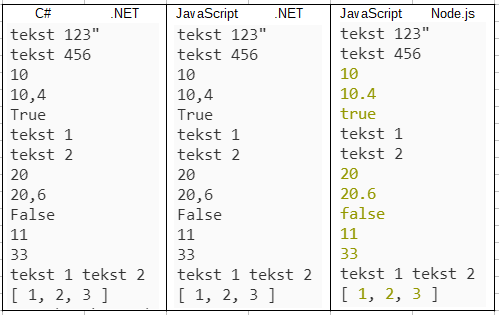
\includegraphics[width=0.7\linewidth]{t1.png}
	\caption{Wyniki wykonania programu testowego dla modułu obsługi standardowego wyjścia. Źródło: własne}
	\label{fig:result1}
\end{figure}

\par Jak można zauważyć, wynik programu w języku C\# oraz JavaScript kompilowanych na wspólną platformę .NET są identyczne. Tutaj należy również wspomnieć, że standardowa biblioteka C\# nie posiada, żadnej z funkcji pozwalającej na wyświetlenie listy elementów tablicy przy pomocy jednej instrukcji. Tak jak podczas implementacji kompilatora JavaScript została zastosowana tutaj funkcja łącząca elementy tablicy w jeden ciąg znaków oraz zostały doklejone nawiasy otwierające oraz zamykające. 
\par Porównując wynik programu uruchomionego na platformie .NET z programem uruchomionym na platformie Node.js, można zauważyć nie wielkie różnice w wyświetlanych wynikach. Pierwszą z nich rzucającą się w oczy, jest zmiana koloru wyświetlanego tekstu dla liczb oraz wartości liczbowych. Jednak ten efekt zależny jest od formatowania kolorów w danej konsoli. Konsola wykryła wywołanie platformy Node.js, dzięki czemu zmieniła kolorystykę.
\par Drugim z różniącym się elementem jest sposób wyświetlania liczb rzeczywistych. Różnią się tym, że dla platformy .NET wyświetlany jest przecinek, kiedy na platformie Node.js wyświetlana jest kropka. Ostatnią różnicą w prezentowanych wynikach jest wyświetlanie wartości logicznych. Dla platformy .NET wartości są wyświetlane z wielką literą, a w przypadku Node.js wartości wyświetlane są małymi literami.

\par Kolejnym z testów dla którego wynik wykonania programu był różny, został przeprowadzony dla modułu działań arytmetycznych. Zrzuty wyników zostały przedstawione na rysunku \ref{fig:result2}. Głównie różnice występują przy wyświetlaniu wyniku operacji dzielenia.

\begin{figure}[!h]
	\centering
  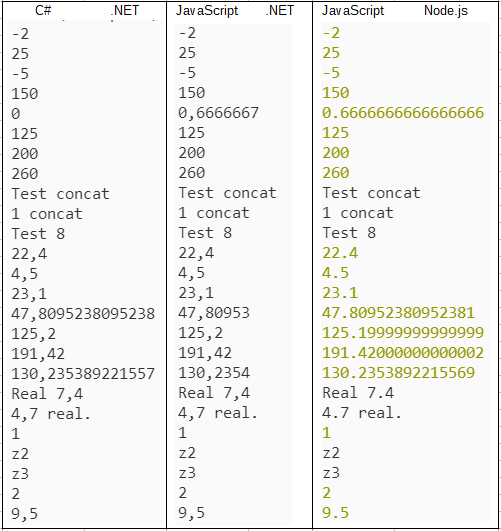
\includegraphics[width=0.7\linewidth]{t2.png}
	\caption{Wyniki wykonania programu testowego dla modułu obsługi działania arytmetyczne. Źródło: własne}
	\label{fig:result2}
\end{figure}

\par Pierwszą z różnic między programem napisanym w języku C\# a JavaScript na platformie .NET jest wynik dzielenia dwóch liczb całkowitych. Wykonywane działanie ma postać $y = 10 / 15$, więc wynikiem jest liczba rzeczywista. W programie w języku C\# jest językiem silnie typowanym, co oznacza, że jeżeli przynajmniej jedna z liczb nie zostanie przekonwertowana na typ liczb rzeczywistych, to wynik będzie typu liczby całkowitej. W tworzonym kompilatorze została zaimplementowana automatyczna konwersja typów, w momencie kiedy zostanie wykryta operacja dzielenia dwóch liczb.
\par Drugą z widocznych różnic jest precyzja wartości zmiennych. W tworzonym kompilatorze JavaScript został wykorzystany typ pojedynczej precyzji, a w przypadku kompilatora C\# została zastosowana typ podwójnej precyzji. Porównując wyniki platformy .NET do platformy Node.js można zauważyć, że wartości na platformie .NET są zaokrąglane.

\par Przy uruchomieniu programu JScript jednego z algorytmów testujących, ukazała się jeszcze jedna różnica w prezentowanych na konsoli wynikach. Różnicą jest sposób wyświetlania tablicy elementów. W tworzonym kompilatorze, jak i na platformie .NET, elementy są otoczone nawiasem kwadratowym, oraz oddzielone są poza przecinkiem dodatkową spacją. W przypadku wyniku programu JScript, prezentowana tablica nie posiada nawiasów kwadratowych oraz liczby są oddzielone przecinkami bez spacji. Wynik programów zaprezentowany jest na rysunki \ref{fig:result3}

\begin{figure}[!h]
	\centering
  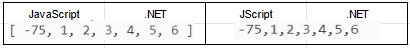
\includegraphics[width=0.7\linewidth]{t3.png}
	\caption{Wyniki wykonania programu dla algorytmu testowego nr 1. Źródło: własne}
	\label{fig:result3}
\end{figure}

\par Skrypty testowe dla pozostałych modułów nie wykazują różnic w prezentowanych wynikach na konsoli.

\subsection{Porównanie generowanego kodu assemblera}

\par Generowany kod assemblera z języka JavaScript będzie porównany z kodem dezasemblowanym kodem programu napisanego w języku C\#. Dezasemblacja jest wykonywana przy pomocy programu \textit{ildasm.exe} znajdujący się w pakiecie \textbf{.NET Framework}.
\par Pierwszą z widocznych różnic jest ilość deklaracji metadanych w nagłówku pliku. Kolejną z różnic jest ilość modyfikatorów przy deklaracji klasy jak i metody \texttt{Main}. Dla deklaracji klasy programu C\# zostały użyte następujące słowa kluczowe \texttt{private}, \texttt{auto}, \texttt{ansi}, \texttt{beforefieldinit}, a dla funkcji \texttt{Main} zostały użyte: \texttt{private} oraz \texttt{hidebysig}. 

\begin{figure}[!h]
	\centering
  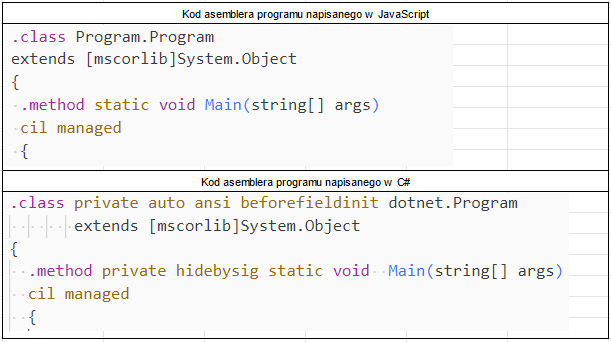
\includegraphics[width=0.9\linewidth]{t4.png}
	\caption{Porównanie kodu asemblera dla deklaracji klasy oraz funkcji \texttt{Main}. Źródło: własne}
	\label{fig:result4}
\end{figure}

\par Kolejnym z różnic jest ilość deklarowanych zmiennych, która spowodowana jest słabą optymalizacją w tworzonym kompilatorze. Następną rzeczą jest nadawanie etykiet dla każdej z instrukcji w obrębie deklarowanych funkcji. 

\par Analizując generowane instrukcje kodu asemblera z dezasemblowanym kodem programu C\# można zauważyć różnicę przy zapisywaniu oraz odczytywaniu wartości zmiennych na stosie. W utworzonym kompilatorze odbywa się to zawsze poprzez nazwę zmiennej, a w .NET Framework wykorzystywane są instrukcje wykorzystujące indeksowanie zmiennych od wartości 0 do 3. Dodatkowo odwołanie się do kolejnych zmiennych wykorzystywana jest instrukcja w formie skróconej.


\begin{lstlisting}[language=IL, caption={Fragment kodu deasemblerowanego testu programu C\#, przedstawiający ładowanie wartości zmiennych na stos}, label=alg:asm]
  ...
  IL_0047:  ldloc.0
  IL_0048:  call       void [mscorlib]System.Console::WriteLine(string)
  IL_004d:  ldloc.1
  IL_004e:  call       void [mscorlib]System.Console::WriteLine(string)
  IL_0053:  ldloc.2
  IL_0054:  call       void [mscorlib]System.Console::WriteLine(int32)
  IL_0059:  ldloc.3
  IL_005a:  call       void [mscorlib]System.Console::WriteLine(float32)
  IL_005f:  ldloc.s    V_4
  IL_0061:  call       void [mscorlib]System.Console::WriteLine(bool)
  ...
\end{lstlisting}

\par Następne różnice generowanego kodu widoczne są przy operacjach arytmetycznych, wykonywanych na liczbach stałych. W przypadku wykorzystania \textit{.NET Framework}, obliczenia wykonywane są przy generowaniu kodu, a nie podczas uruchomienia skompilowanego programu. Przykładowo wykonanie działania $x = 1 + 2$, wygeneruje instrukcje jedynie do przypisania wartości $3$ do zmiennej $x$. W tworzonym kompilatorze, wygenerowanie zostanie instrukcji do załadowania liczby $1$ oraz $2$ na stos, następnie wykonanie operacji dodawania i na końcu przypisanie wyniku do zmiennej $x$.
\par Przy dodawaniu do siebie wielu łańcuchów znaków, w kodzie assemblera, programu napisanego w języku C\#, można zauważyć, że wszystkie łańcuchy są łączone przy pomocy jednej instrukcji \texttt{Concat}, gdzie w tworzonym kompilatorze, zawsze łączone są jedynie dwa łańcuchy na raz. Co więcej, można zauważyć też różnicę przy konwersji wartości zmiennych na łańcuchy znaków przy dodawaniu ich do elementów typu łańcuchowego. W tworzonym kompilatorze konwersja przebiega przy pomocy instrukcji \texttt{ToString()}, jednak w kompilatorze środowiska \textit{.NET Framework} przeprowadzana jest przy pomocy instrukcji \texttt{box}, która sprowadza zmienną do typu \texttt{object}. Instrukcja \texttt{Concat} przyjmuje wtedy elementy typu \texttt{object}.

\begin{lstlisting}[language=IL, caption={Fragment kodu deasemblerowanego testu programu C\#, przedstawiający łączenie łańcuchów znaków}, label=alg:asm]
  ...
  IL_006a:  ldloc.s    V_1
  IL_006c:  ldc.i4.2
  IL_006d:  box        [mscorlib]System.Int32
  IL_0072:  ldstr      "Tekst"
  IL_0077:  call       string [mscorlib]System.String::Concat(object,
                                                              object,
                                                              object)
  ...
\end{lstlisting}

\par Dalej analizując poszczególne moduły, można zauważyć, że w generowanym kodzie assemblera dla programów kompilowanych przy pomocy narzędzi środowiska \textit{.NET Framework}, naturalnie wykorzystywane są wszystkie dostępne instrukcje. Szczególnie widoczne jest to przy instrukcjach warunkowych. W tworzonym kompilatorze warunki zawsze są sprowadzane do pojedynczej wartości logicznej, a następnie na jej podstawie wykonywany jest skok. W przypadku kompilatora \textit{.NET}, przykładowo wykorzystywane są instrukcje które od razu porównują dwie wartości na jej podstawie wykonują skok.

\begin{lstlisting}[language=IL, caption={Fragment kodu deasemblerowanego testu programu C\#, przedstawiający instrukcje \texttt{if ... else}}, label=alg:asm]
  ...
  IL_0060:  ldc.i4.s   20
  IL_0062:  ldloc.s    number1
  IL_0064:  ble.s      IL_0072

  IL_0066:  ldstr      "number1 is less than 20"
  IL_006b:  call       void [mscorlib]System.Console::WriteLine(string)
  IL_0070:  br.s       IL_007c

  IL_0072:  ldstr      "number1 is greater than 20"
  IL_0077:  call       void [mscorlib]System.Console::WriteLine(string)
  IL_007c:  
  ...
\end{lstlisting}

\begin{lstlisting}[language=IL, caption={Fragment wygenerowanego kodu asemblerowanego z języka JavaScript, przedstawiający instrukcje \texttt{if ... else}}, label=alg:asm]
  ...
  ldc.i4 20
  ldloc v_number1
  cgt
  stloc v_tmp_11
  // BOOLEAN:tmp_11 = INTEGER:20 > INTEGER:number1
  
  ldloc v_tmp_11
  brfalse IF_2
  // if (BOOLEAN:tmp_11 == false) JUMP IF_2
  ldstr "number1 is less than 20"
  call void [mscorlib]System.Console::WriteLine(string)
  
  br IF_3
  IF_2: 
  // ELSE
  ldstr "number1 is greater than 20"
  call void [mscorlib]System.Console::WriteLine(string)
  ...
\end{lstlisting}

% w pętlach jest inna kolejność instrukcji
% \subsection{Porównanie zdekompilowanego kodu programu w postaci języka C\#}

\section{Testy algorytmów}

\par W celu przetestowania działania tworzonego kompilatora, zostały wykorzystane algorytmy odnalezione w Internecie. Zostaną dla nich utworzone odpowiednie kody w języku C\# w celu porównania szybkości działania, zużycia pamięci czy wykorzystania przestrzeni dyskowej. Dla kodu programu w JavaScript zostaną również utworzone wersje przystosowane do kompilatora JScript, którego wyniki również zostaną porównane.

\subsection{Algorytm sortowania}
\par Pierwszym z odnalezionych kodów jest algorytm sortowania bąbelkowego zamieszczony w artykule zamieszczonego pod adresem \url{https://www.educba.com/sorting-algorithms-in-javascript/}, którego autorem jest Priya Pedamkar. Kod przedstawia się następująco:

\begin{lstlisting}[language=JavaScript, caption={Algorytm sortowania bąbelkowego. Źródło: \url{https://www.educba.com/sorting-algorithms-in-javascript/}}, label=alg:alg1]
function swap(arr, firstIndex, secondIndex){
  var temp = arr[firstIndex];
  arr[firstIndex] = arr[secondIndex];
  arr[secondIndex] = temp;
}
function bubbleSortAlgo(arraaytest){
  var len = arraaytest.length,
  i, j, stop;
  for (i=0; i < len; i++){
    for (j=0, stop=len-i; j < stop; j++){
      if (arraaytest[j] > arraaytest[j+1]){
        swap(arraaytest, j, j+1);
      }
    }
  }
  return arraaytest;
}
console.log(bubbleSortAlgo([3, 6, 2, 5, -75, 4, 1]));
\end{lstlisting}

\par Niestety funkcjonalność obsługi tablic nie została w pełni zaimplementowana, co powoduje, że powyższy kod dla stworzonego kompilatora nie jest poprawny. Problem występuje w dwóch miejscach. Pierwszy z nich znajduje się w wewnętrznej instrukcji \texttt{for} a dokładniej w warunku kończącym iterowanie pętli. W języku JavaScript przy odwołaniu się do elementu poza zakresem tablicy, nie zostanie wywołany błąd a jedynie zostanie zwrócona wartość typu \texttt{undefined}. W środowisku \textit{.NET Framework} wyjście poza zakres powoduje błąd i zatrzymanie działania programu. W celu uniknięcia tego, zmienna \texttt{stop} została zmniejszona o $1$. 
\par Drugim miejscem jest wywołanie funkcji, podając dla niej bezpośrednio tablicę wartości. Problem polega na braku obsłużenia przedstawionej sytuacji, w której przekazywane jest bezpośrednio nowo utworzona tablica elementów, co skutkuje wygenerowaniem błędnego kodu asemblera, którego po skompilowaniu do postaci binarnej, uruchomienie powoduje błąd środowiska maszyny wirtualnej. Aby uniknąć tego błędu, nowo tworzona tablica będzie najpierw przypisana do zmiennej, a dopiero następnie przekazana do funkcji.

\begin{lstlisting}[language=JavaScript, caption={Zmodyfikowany kod programu sortowania bąbelkowego.}, label=alg:alg1]
  function swap(arr, firstIndex, secondIndex){
    var temp = arr[firstIndex];
    arr[firstIndex] = arr[secondIndex];
    arr[secondIndex] = temp;
  }
  function bubbleSortAlgo(arraaytest){
    var len = arraaytest.length,
    i, j, stop;
    for (i=0; i < len; i++){
      for (j=0, stop=len - i - 1; j < stop; j++){
        if (arraaytest[j] > arraaytest[j+1]){
          swap(arraaytest, j, j+1);
        }
      }
    }
    return arraaytest;
  }
  var l = [3, 6, 2, 5, -75, 4, 1];
  console.log(bubbleSortAlgo(l));
\end{lstlisting}

\par W celu skompilowania powyższego kodu algorytmu przy pomocy kompilatora JScript z pakietu \textit{.NET Framework}, wystarczy jedynie dodać instrukcje importujące biblioteki standardowe \texttt{System} oraz \texttt{Microsoft.Win32}. Instrukcje należy umieścić na początku pliku. Kolejną konieczną rzeczą do skompilowania kodu, jest zmiana instrukcji standardowego wyjścia. Instrukcja \texttt{console.log(...)} powinna być zastąpiona instrukcją \texttt{Console.WriteLine(...)}. Tak przygotowany kod źródłowy można teraz skompilować kompilatorem JScript.

\par Kod JavaScript został odwzorowany również w kodzie C\# i prezentuje się następująco:

\begin{lstlisting}[language=CSharp, caption={Odwzorowany kod JavaScript w języku C\# algorytmu sortowania bąbelkowego.}, label=alg:alg1]
using System;
using System.Collections.Generic;

namespace dotnet
{
  class Program
  {
    static void swap(List<int> arr, int firstIndex, int secondIndex)
    {
      int temp = arr[firstIndex];
      arr[firstIndex] = arr[secondIndex];
      arr[secondIndex] = temp;
    }

    static List<int> bubbleSortAlgo(List<int> arraaytest)
    {
      int len = arraaytest.Count, i, j, stop;
      for (i = 0; i < len; i++)
      {
        for (j = 0, stop = len - i - 1; j < stop; j++)
        {
          if (arraaytest[j] > arraaytest[j + 1])
          {
            swap(arraaytest, j, j + 1);
          }
        }
      }
      return arraaytest;
    }

    static void Main(string[] args)
    {
      List<int> l = new List<int>() { 3, 6, 2, 5, -75, 4, 1 };
      Console.WriteLine("[ "+string.Join(", ", bubbleSortAlgo(l))+" ]");
    }
  }
}
\end{lstlisting}

\par Testy zostaną wykonane dla oryginalnego wektora wejściowego do przesortowania jak i dla losowo wygenerowanego wektora o wielkościach 1000, 5000 i 10000 składającego się z liczb całkowitych z przedziału od -10000 do 10000.

\par Pierwszym z kryteriów jest zmierzenie czasu wykonywania programu. Czas zmierzony będzie w w konsoli \textit{PowerShell 7.1.1} przy pomocy komendy \texttt{Measure-Command} uruchamiającego proces skompilowanego pliku programu. Otrzymane wyniki prezentują się następująco:

\begin{table}[h!]
  \begin{tabular}{|l|l|l|l|}
  \hline
  Ilość elementów & C\#              & JavaScript       & JScript          \\ \hline
  Oryginalne (7)  & 00:00:01.0280485 & 00:00:01.0211699 & 00:00:01.0249265 \\ \hline
  1000            & 00:00:01.0267120 & 00:00:01.0209711 & 00:00:01.0281652 \\ \hline
  5000            & 00:00:01.0231339 & 00:00:01.0286513 & 00:00:11.1320074 \\ \hline
  10000           & 00:00:01.0331534 & 00:00:01.0466795 & 00:00:47.3928596 \\ \hline
  \end{tabular}
\end{table}

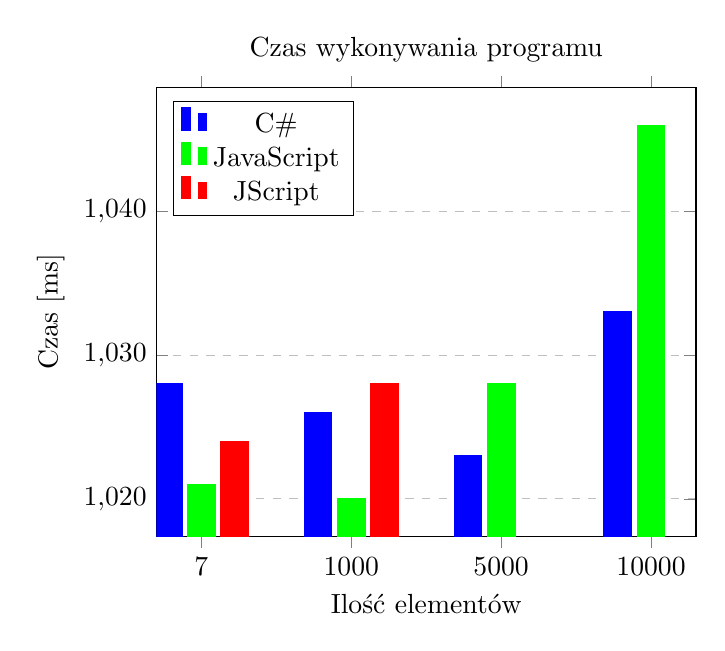
\begin{tikzpicture}
  \begin{axis}[
      ybar,
      title={Czas wykonywania programu},
      xlabel={Ilość elementów},
      ylabel={Czas [ms]},
      symbolic x coords={7,1000,5000,10000},
      xtick=data,
      legend pos=north west,
      ymajorgrids=true,
      grid style=dashed,
      % nodes near coords
  ]
  
  \addplot[
      color=blue,
      fill=blue
    ]
    coordinates {
      (7, 1028)
      (1000,1026)
      (5000,1023)
      (10000,1033)
    };
    \addlegendentry{C\#}

    
  \addplot[
    color=green,
    fill=green
    ]
    coordinates {
      (7,1021)
      (1000,1020)
      (5000,1028)
      (10000,1046)
    };
    \addlegendentry{JavaScript}

    
  \addplot[
      color=red,
      fill=red,
    ]
    coordinates {
      (7,1024)
      (1000,1028)
    };
    \addlegendentry{JScript}
      
  \end{axis}
\end{tikzpicture}

\par Obserwując wyniki pomiarów czasu wykonywania programu, można stwierdzić, że utworzony kompilator jest porównywalny do kompilatora C\#. W przypadku kompilatora JScript różnicę można zauważyć przy większej ilości danych. W przypadku kiedy wektor testowy miał 5000 elementów, czas wykonywania programu zwiększył się średnio o 10 sekund, a w przypadku kiedy wektor testowy posiadał 10000 elementów, czas wykonania osiągną średnio 47 sekund.

\par Kolejnym z kryteriów jest sprawdzenie wykorzystania pamięci dla programów testowych. Zostanie do tego wykorzystane narzędzie \textit{JetBrains dotMemory 2020.2.1}. Test zostanie wykonany dla programów z wektorem wejściowym posiadającym 10000.

\begin{table}[h!]
  \centering
  \begin{tabular}{|l|l|}
  \hline
  Kompilator & Zużycie pamięci \\ \hline
  C\# & 11,26 MB \\ \hline
  JavaScript & 11,25 MB \\ \hline
  JScript & 28,72 MB \\ \hline
  \end{tabular}
\end{table}

\begin{figure}[!h]
  \centering
  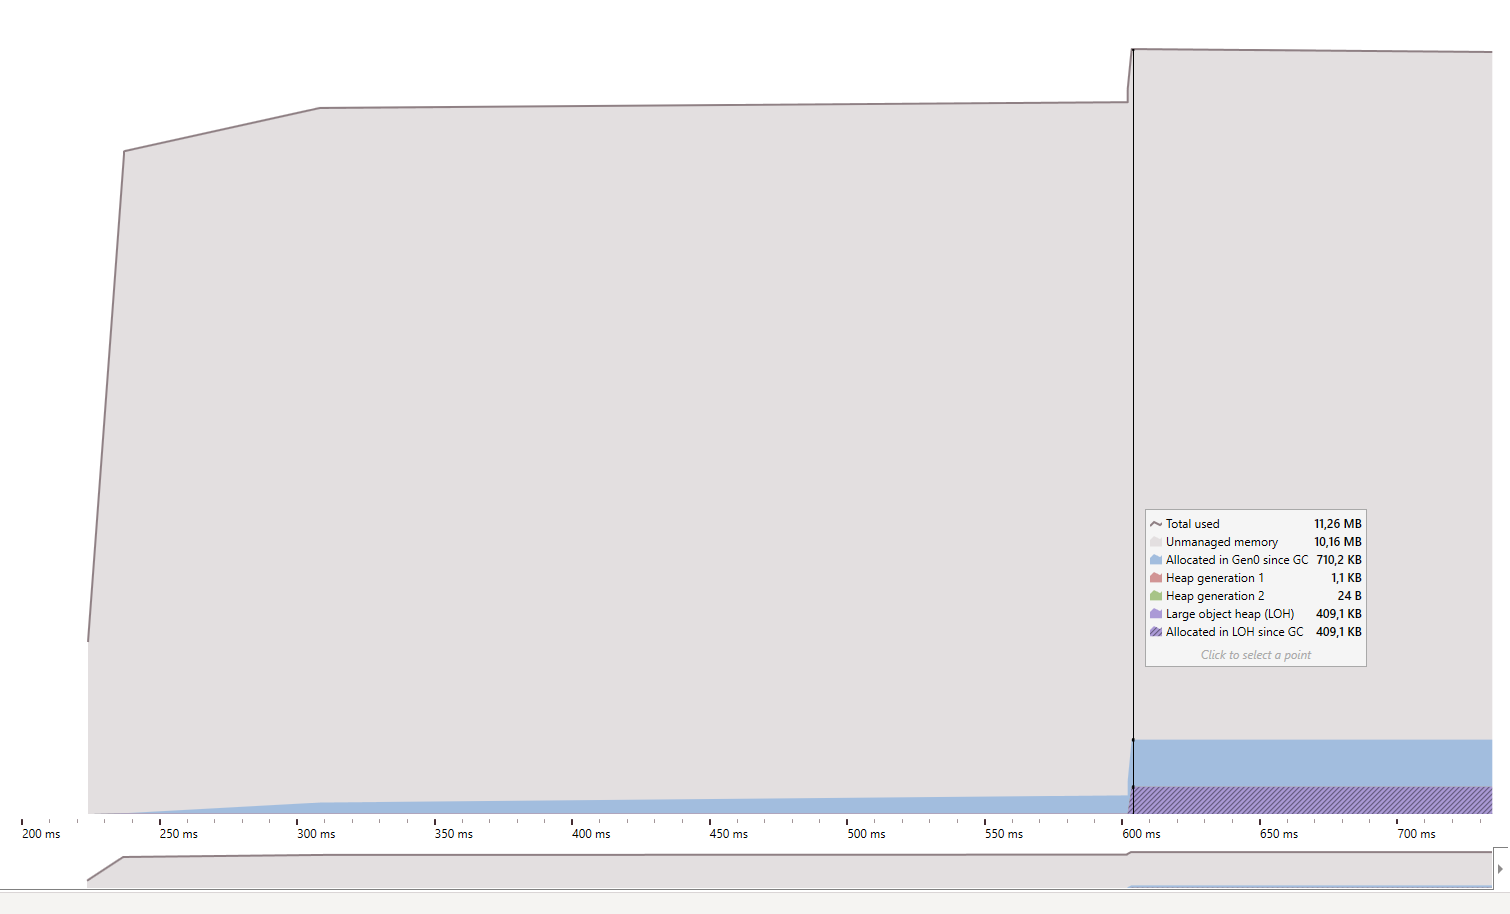
\includegraphics[width=0.75\linewidth]{a1_cs_10000.png}
  \caption{Pomiar zużycia pamięci dla algorytmu pierwszego dla kompilatora C\#. Źródło: własne}
  \label{fig:a}
\end{figure}

\begin{figure}[!h]
  \centering
  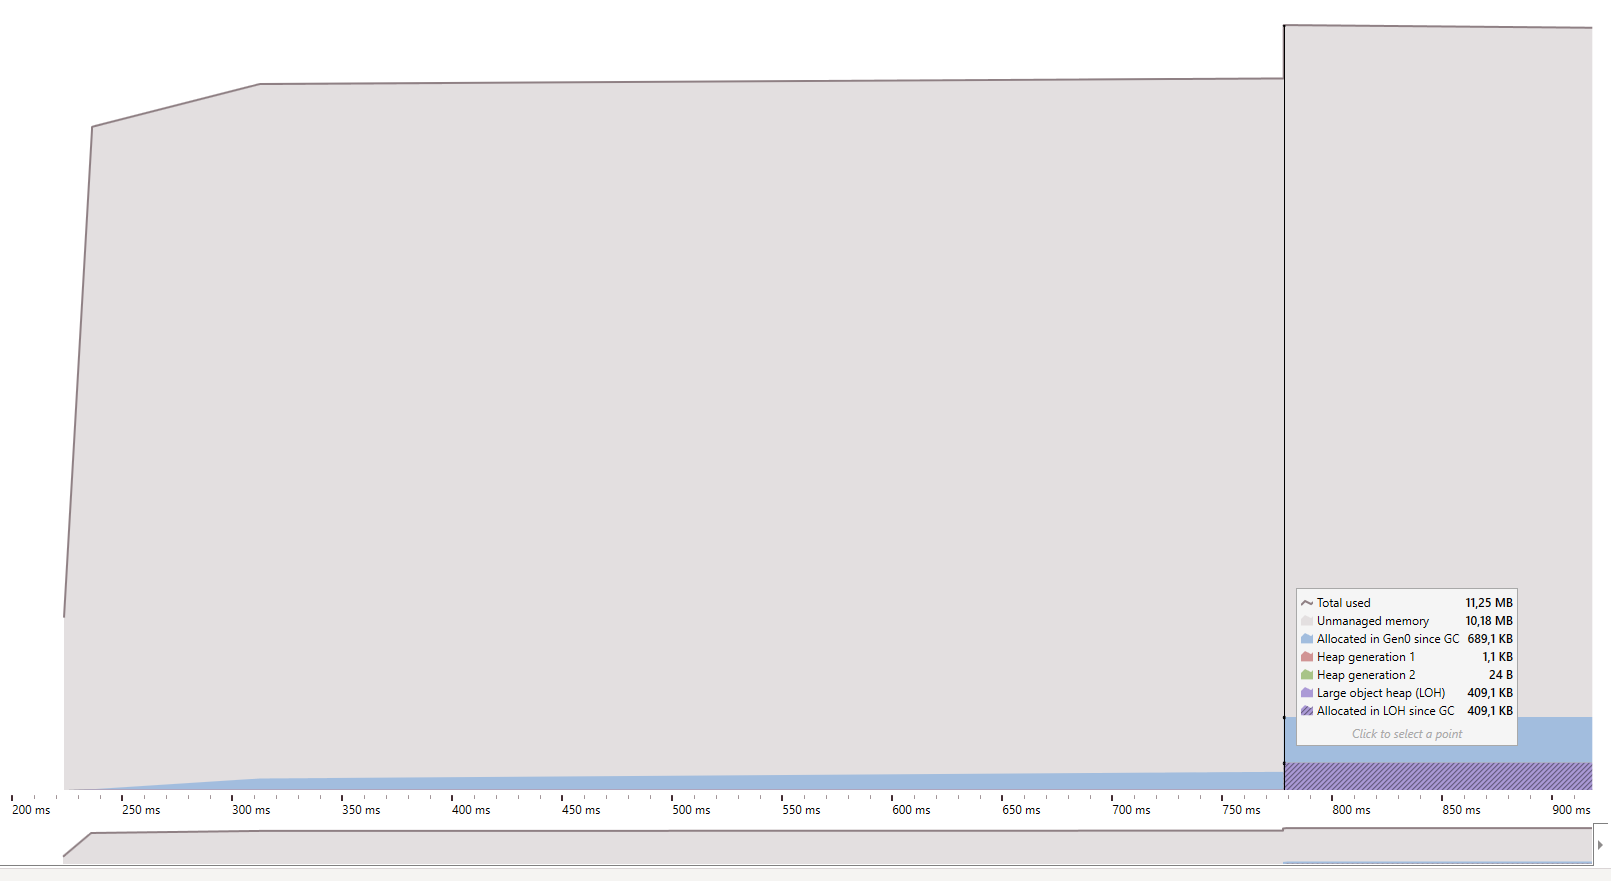
\includegraphics[width=0.75\linewidth]{a1_js_10000.png}
  \caption{Pomiar zużycia pamięci dla algorytmu pierwszego dla kompilatora JavaScript. Źródło: własne}
  \label{fig:a}
\end{figure}

\begin{figure}[!h]
  \centering
  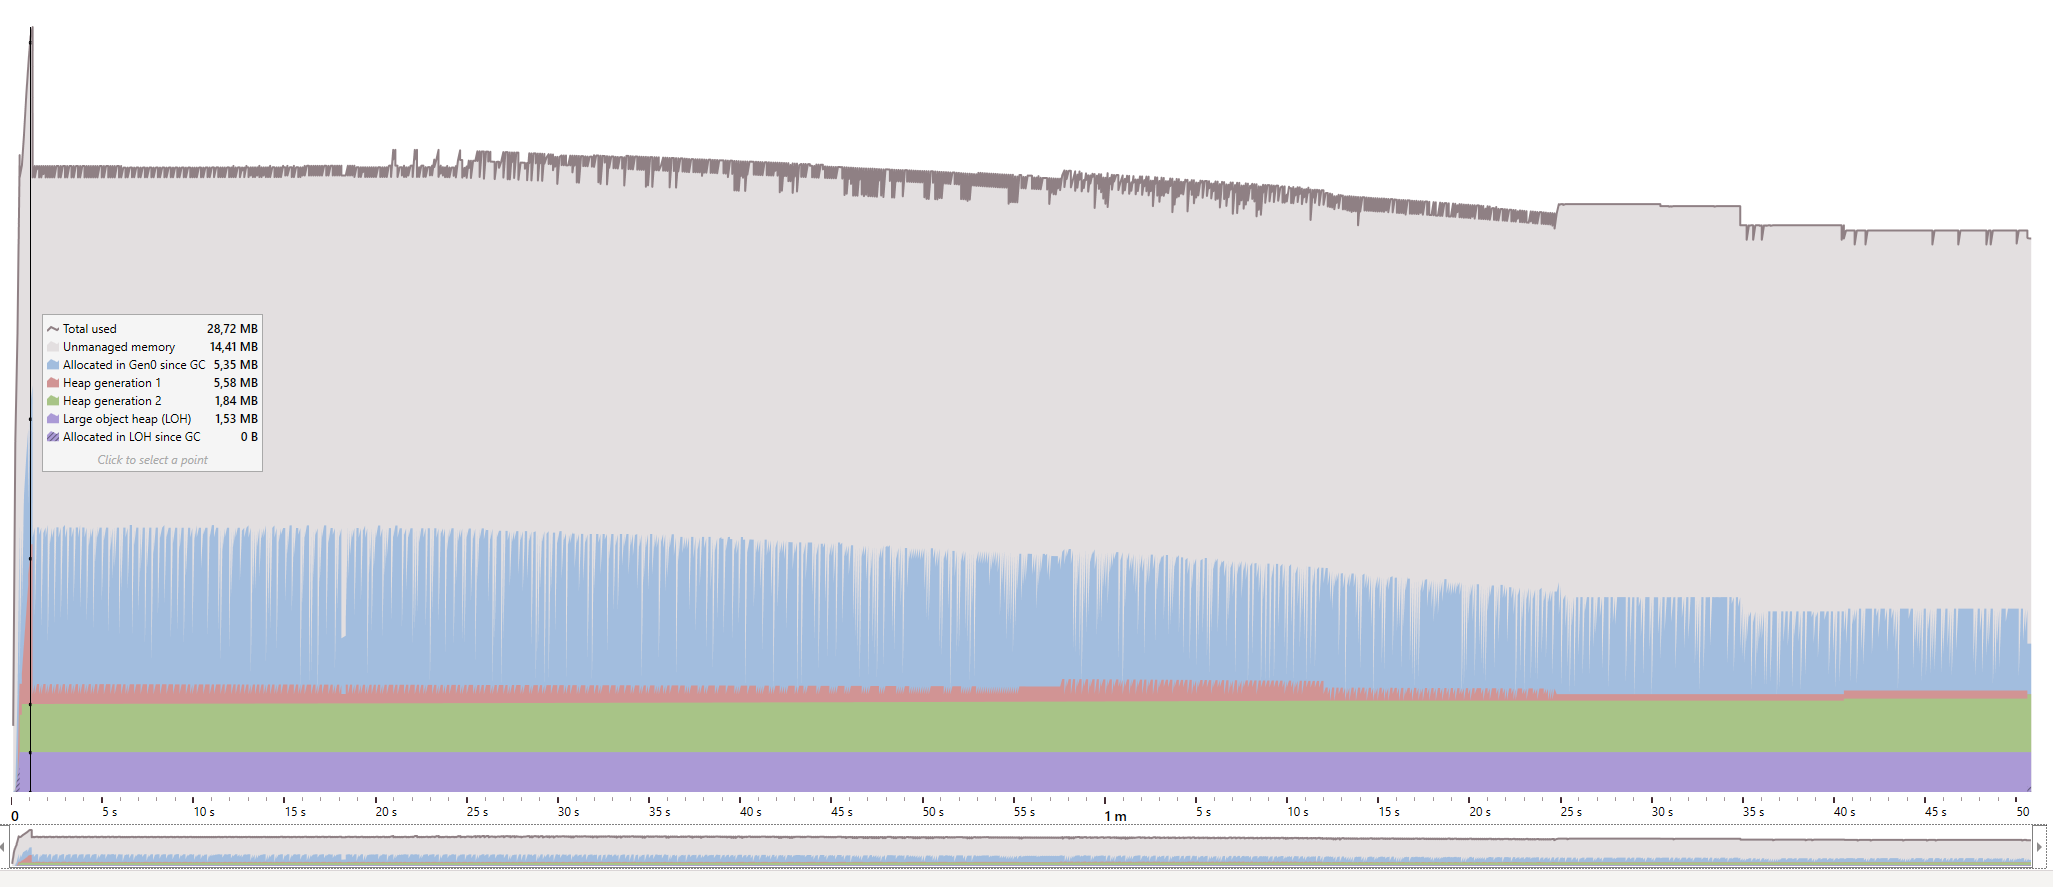
\includegraphics[width=0.75\linewidth]{a1_jsm_10000.png}
  \caption{Pomiar zużycia pamięci dla algorytmu pierwszego dla kompilatora JScript. Źródło: własne}
  \label{fig:a}
\end{figure}

\newpage
\par Tak ja w poprzednim teście, wyniki pokazują, że pomiędzy programem C\# oraz programem JavaScript nie występuje znaczna różnica. Inaczej jest z programem JScript który zużywa w piku ponad dwukrotnie więcej pamięci.

\par Ostatnim z kryteriów jest zmierzenie wielkości plików skompilowanych programów. Wyniki prezentują się następująco:

\begin{table}[h!]
  \begin{tabular}{|l|l|l|l|}
  \hline
  Ilość elementów & C\#              & JavaScript       & JScript          \\ \hline
  Oryginalne (7)  & 4,00 kB & 3,00 kB & 7,00 kB \\ \hline
  1000            & 15,00 kB & 16,50 kB & 23,00 kB \\ \hline
  5000            & 57,50 kB & 71,00 kB & 89,50 kB \\ \hline
  10000           & 111,00 kB & 139,50 kB & 172,00 kB \\ \hline
  \end{tabular}
\end{table}


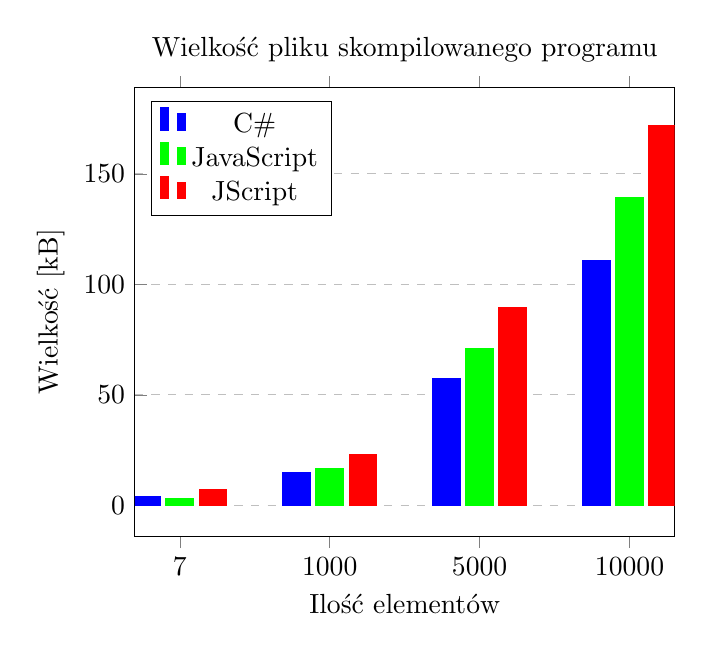
\begin{tikzpicture}
  \begin{axis}[
      ybar,
      title={Wielkość pliku skompilowanego programu},
      xlabel={Ilość elementów},
      ylabel={Wielkość [kB]},
      symbolic x coords={7,1000,5000,10000},
      xtick=data,
      legend pos=north west,
      ymajorgrids=true,
      grid style=dashed,
      % nodes near coords
  ]
  
  \addplot[
      color=blue,
      fill=blue
    ]
    coordinates {
      (7, 4.00)
      (1000,15.00)
      (5000,57.50)
      (10000,111.00)
    };
    \addlegendentry{C\#}

    
  \addplot[
    color=green,
    fill=green
    ]
    coordinates {
      (7,3.00)
      (1000,16.50)
      (5000,71.00)
      (10000,139.50)
    };
    \addlegendentry{JavaScript}

    
  \addplot[
      color=red,
      fill=red,
    ]
    coordinates {
      (7,7.00)
      (1000,23.00)
      (5000,89.50)
      (10000,172.00)
    };
    \addlegendentry{JScript}
      
  \end{axis}
\end{tikzpicture}




% \subsection{Algorytm wyszukiwania}

% 1. Obsługa standardowego wyjścia
% 2. Obsługa zmiennych
% 3. Obsługa działań arytmetycznych
% 4. Obsługa wyrażeń warunkowych
% 5. Obsługa pętli
% 6. Obsługa tablic
% 7. Obsługa funkcji


%----------------------------------------------------------------------------------------
%	ROZDZIAŁy kolejne należy dodać analogicznie do 1 i 2 
% utworzyć pliki i je załączyć (include)
%----------------------------------------------------------------------------------------

%----------------------------------------------------------------------------------------
%	ZAKOŃCZENIE PRACY DYPLOMOWEJ (JK - design and implementation)
%----------------------------------------------------------------------------------------
\addcontentsline{toc}{chapter}{Podsumowanie}
%%%%%%%%%%%%%%%%%%%%%%%%%%%%%%%%%%%%%%%%%
% Wnioski do pracy dyplomowej
% Szablon pracy dyplomowej
% Wydział Informatyki 
% Zachodniopomorski Uniwersytet Technologiczny w Szczecinie
% autor Joanna Kołodziejczyk (jkolodziejczyk@zut.edu.pl)
% Bardzo wczesnym pierwowzorem szablonu był
% The Legrand Orange Book
% Version 2.1 (26/09/2018)
%
% Modifications to LOB assigned by %JK
%%%%%%%%%%%%%%%%%%%%%%%%%%%%%%%%%%%%%%%%%


\chapter*{Podsumowanie}

Podsumowanie pracy powinno na maksymalnie dwóch stronach przedstawić główne wyniki pracy dyplomowej. Struktura zakończenia to:
\begin{enumerate}
\item Przypomnienie celu i hipotez
\item Co w pracy wykonano by cel osiągnąć (analiza, projekt, oprogramowanie, badania eksperymentalne)
\item Omówienie głównych wyników pracy
\item Jak wyniki wzbogacają dziedzinę
\item Zamknięcie np. poprzez wskazanie dalszych kierunków badań.
\end{enumerate} % conclusions.tex zawiera treść zakończenia/podsumowania pracy dyplomowej


%----------------------------------------------------------------------------------------
%	SPIS LITERATURY (JK - design and implementation)
%----------------------------------------------------------------------------------------
\pagestyle{empty} 
\chapter*{Spis literatury}
\addcontentsline{toc}{chapter}{\textcolor{blueZUT}{Spis literatury}}
% Poniżej zdefiniowane są filtry do dzielenia spisu literatury na kategorie
\defbibfilter{articles}{
  type=article or 
  type=inproceedings
}
\defbibfilter{other}{
  type=url or
  type=online  or
  type=manual or
  type=misc
}

% UWAGA! -aby zmienić zawartość spisu literatury należy wyedytować plik
% bibliography.bib

%------------------------------------------------
% Spis literartury podzielony jest na 3 kategorie
% 1
\section*{Książki}
\addcontentsline{toc}{section}{Książki}
\printbibliography[heading=bibempty,type=book]

%------------------------------------------------
% 2
\section*{Artykuły}
\addcontentsline{toc}{section}{Artykuły}
\printbibliography[heading=bibempty,filter=articles]
%------------------------------------------------
% 3
\section*{Źródła internetowe i inne}
\addcontentsline{toc}{section}{Źródła internetowe i inne}
\printbibliography[heading=bibempty,filter=other]


%----------------------------------------------------------------------------------------
%	APPENDIX (JK - design and implementation)
%----------------------------------------------------------------------------------------
% \pagestyle{fancy} 
% \begin{appendix}
% \appendix
% %%%%%%%%%%%%%%%%%%%%%%%%%%%%%%%%%%%%%%%%%
% Szablon pracy dyplomowej
% Wydział Informatyki 
% Zachodniopomorski Uniwersytet Technologiczny w Szczecinie
% autor Joanna Kołodziejczyk (jkolodziejczyk@zut.edu.pl)
% Bardzo wczesnym pierwowzorem szablonu był
% The Legrand Orange Book
% Version 2.1 (26/09/2018)
%
% Modifications to LOB assigned by %JK
%%%%%%%%%%%%%%%%%%%%%%%%%%%%%%%%%%%%%%%%%


\chapter{Dodatek}
\label{chapter:dodatek_A}

\textit{W dodatkach mogą znaleźć się większe fragmenty kodów źródłowych, instrukcje działania programów, specyfikacje opcji, z którymi wywołuje się program, większe dane tabelaryczne, specyfikacje oprogramowania, dłuższe opisy teoretyczne, itp.}

What is Lorem Ipsum?
Lorem Ipsum is simply dummy text of the printing and typesetting industry. Lorem Ipsum has been the industry'es standard dummy text ever since the 1500s, when an unknown printer took a galley of type and scrambled it to make a type specimen book. It has survived not only five centuries, but also the leap into electronic typesetting, remaining essentially unchanged. It was popularised in the 1960s with the release of Letraset sheets containing Lorem Ipsum passages, and more recently with desktop publishing software like Aldus PageMaker including versions of Lorem Ipsum.

Why do we use it?
It is a long established fact that a reader will be distracted by the readable content of a page when looking at its layout. The point of using Lorem Ipsum is that it has a more-or-less normal distribution of letters, as opposed to using 'Content here, content here', making it look like readable English. Many desktop publishing packages and web page editors now use Lorem Ipsum as their default model text, and a search for 'lorem ipsum' will uncover many web sites still in their infancy. Various versions have evolved over the years, sometimes by accident, sometimes on purpose (injected humour and the like).


Where does it come from?
Contrary to popular belief, Lorem Ipsum is not simply random text. It has roots in a piece of classical Latin literature from 45 BC, making it over 2000 years old. Richard McClintock, a Latin professor at Hampden-Sydney College in Virginia, looked up one of the more obscure Latin words, consectetur, from a Lorem Ipsum passage, and going through the cites of the word in classical literature, discovered the undoubtable source. Lorem Ipsum comes from sections 1.10.32 and 1.10.33 of "de Finibus Bonorum et Malorum" (The Extremes of Good and Evil) by Cicero, written in 45 BC. This book is a treatise on the theory of ethics, very popular during the Renaissance. The first line of Lorem Ipsum, "Lorem ipsum dolor sit amet..", comes from a line in section 1.10.32.

The standard chunk of Lorem Ipsum used since the 1500s is reproduced below for those interested. Sections 1.10.32 an

What is Lorem Ipsum?
Lorem Ipsum is simply dummy text of the printing and typesetting industry. Lorem Ipsum has been the industry's standard dummy text ever since the 1500s, when an unknown printer took a galley of type and scrambled it to make a type specimen book. It has survived not only five centuries, but also the leap into electronic typesetting, remaining essentially unchanged. It was popularised in the 1960s with the release of Letraset sheets containing Lorem Ipsum passages, and more recently with desktop publishing software like Aldus PageMaker including versions of Lorem Ipsum.

Why do we use it?
It is a long established fact that a reader will be distracted by the readable content of a page when looking at its layout. The point of using Lorem Ipsum is that it has a more-or-less normal distribution of letters, as opposed to using 'Content here, content here', making it look like readable English. Many desktop publishing packages and web page editors now use Lorem Ipsum as their default model text, and a search for 'lorem ipsum' will uncover many web sites still in their infancy. Various versions have evolved over the years, sometimes by accident, sometimes on purpose (injected humour and the like).


Where does it come from?
Contrary to popular belief, Lorem Ipsum is not simply random text. It has roots in a piece of classical Latin literature from 45 BC, making it over 2000 years old. Richard McClintock, a Latin professor at Hampden-Sydney College in Virginia, looked up one of the more obscure Latin words, consectetur, from a Lorem Ipsum passage, and going through the cites of the word in classical literature, discovered the undoubtable source. Lorem Ipsum comes from sections 1.10.32 and 1.10.33 of "de Finibus Bonorum et Malorum" (The Extremes of Good and Evil) by Cicero, written in 45 BC. This book is a treatise on the theory of ethics, very popular during the Renaissance. The first line of Lorem Ipsum, "Lorem ipsum dolor sit amet..", comes from a line in section 1.10.32.

The standard chunk of Lorem Ipsum used since the 1500s is reproduced below for those interested. Sections 1.10.32 anWhat is Lorem Ipsum?
Lorem Ipsum is simply dummy text of the printing and typesetting industry. Lorem Ipsum has been the industry's standard dummy text ever since the 1500s, when an unknown printer took a galley of type and scrambled it to make a type specimen book. It has survived not only five centuries, but also the leap into electronic typesetting, remaining essentially unchanged. It was popularised in the 1960s with the release of Letraset sheets containing Lorem Ipsum passages, and more recently with desktop publishing software like Aldus PageMaker including versions of Lorem Ipsum.

Why do we use it?
It is a long established fact that a reader will be distracted by the readable content of a page when looking at its layout. The point of using Lorem Ipsum is that it has a more-or-less normal distribution of letters, as opposed to using 'Content here, content here', making it look like readable English. Many desktop publishing packages and web page editors now use Lorem Ipsum as their default model text, and a search for 'lorem ipsum' will uncover many web sites still in their infancy. Various versions have evolved over the years, sometimes by accident, sometimes on purpose (injected humour and the like).


Where does it come from?
Contrary to popular belief, Lorem Ipsum is not simply random text. It has roots in a piece of classical Latin literature from 45 BC, making it over 2000 years old. Richard McClintock, a Latin professor at Hampden-Sydney College in Virginia, looked up one of the more obscure Latin words, consectetur, from a Lorem Ipsum passage, and going through the cites of the word in classical literature, discovered the undoubtable source. Lorem Ipsum comes from sections 1.10.32 and 1.10.33 of "de Finibus Bonorum et Malorum" (The Extremes of Good and Evil) by Cicero, written in 45 BC. This book is a treatise on the theory of ethics, very popular during the Renaissance. The first line of Lorem Ipsum, "Lorem ipsum dolor sit amet..", comes from a line in section 1.10.32.

The standard chunk of Lorem Ipsum used since the 1500s is reproduced below for those interested. Sections 1.10.32 an % conclusions.tex zawiera treść zakończenia/podsumowania pracy dyplomowej
% \end{appendix}
%----------------------------------------------------------------------------------------
% Koniec dokumentu
\end{document}
